\documentclass[conference,onecolumn]{IEEEtran}
\usepackage[utf8]{inputenc}
\usepackage[T1]{fontenc}
\usepackage{graphicx}
\renewcommand{\ttdefault}{lmtt}
\usepackage{booktabs}
\usepackage{float}
\usepackage{url}
\graphicspath{{figures/}{../docs/diagrams/}{../results/}}

\begin{document}

\title{2IMN10 Architecture of Distributed Systems -- Lab Report, Group GROUP-ID}

\author{\IEEEauthorblockN{Anton Novokhatskyi}
\IEEEauthorblockA{2161699}
\and
\IEEEauthorblockN{Illia Solodkyi}
\IEEEauthorblockA{ID}
\and
\IEEEauthorblockN{Emir SURNAME}
\IEEEauthorblockA{ID}}

\maketitle

% ------------------------------------------------------------------
\section{Phase 1: Architectural Model}

\subsection{Requirements and stakeholders}

The word-count service answers keyword queries over a collection of texts that its developers upload and maintain on the server.

\textbf{Functional requirements.}
\begin{itemize}
  \item \textbf{FR1.} A client sends a keyword and a reference to a text stored on the server; the system returns the exact number of occurrences of that keyword in that text.
  \item \textbf{FR2.} The system reports the most frequently requested keywords (hot keywords), ranked by how often clients have asked for them.
\end{itemize}

\textbf{Non-functional requirements.}
\begin{itemize}
  \item \textbf{NFR1 (latency).} The service answers a request in less than 100~ms, measured on the client side from sending the request to receiving the response.
  \item \textbf{NFR2 (caching).} The system caches the answer to every request in an in-memory database (Redis).
\end{itemize}

\textbf{Stakeholders.}
\begin{itemize}
  \item \textbf{Developers and administrators} develop and maintain the application so that it provides its functionality: they upload the texts, deploy the service, and watch its latency and health in order to scale or repair it.
  \item \textbf{Clients} are the users of the word-count functionality: they issue keyword queries and care about correct counts and fast responses.
\end{itemize}

\subsection{Architecture}



Fig.~\ref{fig:phase1} shows the system in the client-server style. The server is the entity facing the clients and providing the word-count functionality; all the infrastructure is inside the ``logical server'' box. The client sees only a single entry point (one hostname and port) that exposes the service API.

\begin{figure}[!h]
  \centering
  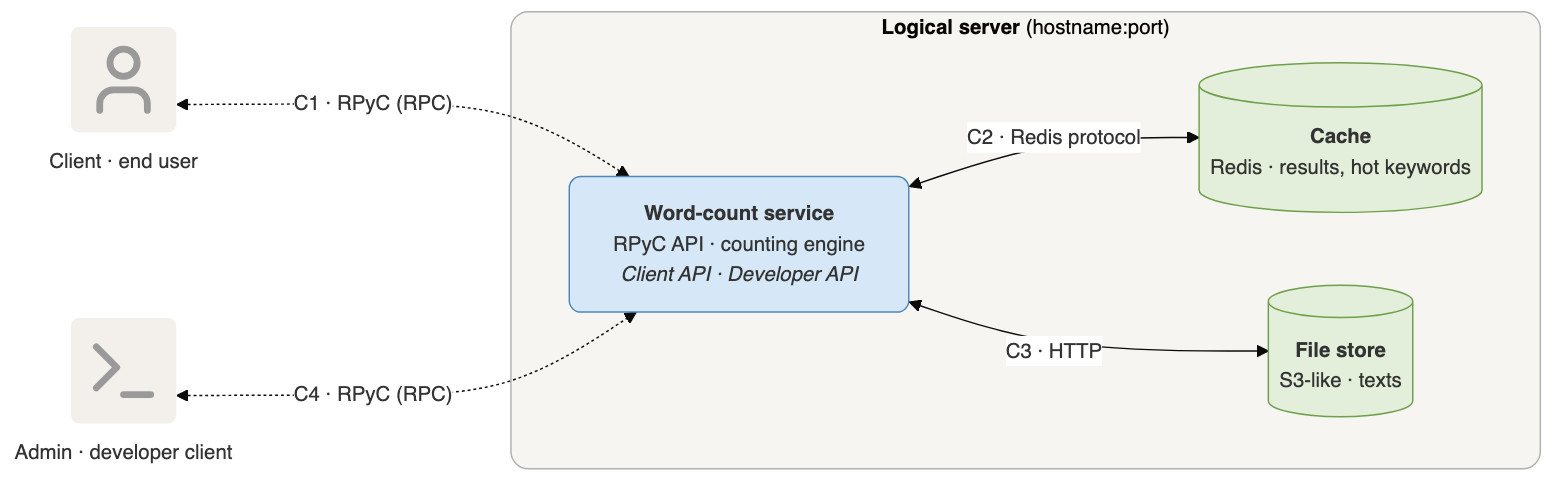
\includegraphics[width=0.7\linewidth]{phase1-mermaid.png}
  \caption{Phase 1 architecture: client-server style. Clients see one logical server; inside it, the word-count service, the cache and the file store.}
  \label{fig:phase1}
\end{figure}

\textbf{Components.}
\begin{itemize}
  \item \textbf{Client:} the user that interacts with the word-count functionality (FR1).
  \item \textbf{Admin (developer client):} maintains the database of texts and inspects usage, through the developer API.
  \item \textbf{Word-count service:} a Python process that exposes the RPC stubs of the service over RPyC and contains the counting engine, i.e.\ the logic of the system given a text.
  \item \textbf{Cache:} Redis, the in-memory database holding the cached counts and the hot-keyword counters (FR2, NFR2).
  \item \textbf{File store:} an S3-like object store holding the texts, the data required for the system to operate; the single source of truth for texts.
\end{itemize}

\textbf{Connectors.} All connectors are synchronous request--reply: the caller waits for the response.
\begin{itemize}
  \item \textbf{C1, C4 -- client/admin $\leftrightarrow$ service:} RPyC remote procedure calls over TCP; a keyword and a text reference travel in, a count (or an error) travels back.
  \item \textbf{C2 -- service $\leftrightarrow$ cache:} Redis protocol; cached counts keyed by (reference, keyword) and the hot-keyword sorted set.
  \item \textbf{C3 -- service $\leftrightarrow$ file store:} HTTP (S3 API); the service fetches a text by its reference on a cache miss.
\end{itemize}

Clients never talk to the cache or the file store, only to the service.

\subsection{Other architectural styles}

When considering the architecture of the application, there are multiple architectural styles. Here we reason how this system might have been implemented using other styles, and what the pros and cons are.

\subsubsection{Peer-to-peer}
The texts are distributed over the peers, and every peer is both a client and a server: it sends queries and counts words in the texts it holds. The peers form a structured overlay using Chord: the reference of each text is hashed to a key, and the peer responsible for that key stores the whole text. There is no central index; the distributed hash table itself is the index, each peer being responsible for a range of keys. A query for a reference is resolved in $O(\log N)$ hops, the responsible peer counts the keyword, and the answer is returned to the peer that asked the query. The super peer is not needed for lookups; it serves as the community access point that new peers contact to discover the overlay and join it.

\noindent\textbf{Pros:} storage. Through resource sharing, the developers do not need to keep additional storage for the system to operate, and the counting work is spread over the peers. No single server is a bottleneck or a single point of failure.

\noindent\textbf{Cons:} latency. The search in a distributed network is slower: a lookup takes up to $O(\log N)$ network hops instead of one call to a known server, and peers that join and leave force keys to move between peers. The hot-keyword ranking (FR2) needs a global view, so it would have to be collected from all peers.

The peer-to-peer architecture is not suitable for this system, and should only be considered if there are strict requirements on the storage.

\subsubsection{Layered}
The client sees the API layer as the entry point, which exposes the service over RPyC. Below it, the service layer contains the counting logic and talks to the data layer, which holds the cache and the file store. This is a strict layered architecture: each layer only calls the layer directly below it, and no upcalls or sidecar are needed. The style is highly suitable, and in fact the internals of our server already follow this strict layered architecture.

\noindent\textbf{Pros:} modifiability. The layered abstraction separates concerns, so a layer can be changed, e.g.\ replacing the cache or the file store, without changing the others, and the layers can be developed concurrently.

\noindent\textbf{Cons:} latency. Every call to a lower layer adds a step to the request, and when the layers run on separate machines each step is a network round trip, so the response time grows with the number of layers.

% ------------------------------------------------------------------
\section{Phase 2: Implementation and Latency Evaluation}

\subsection{Experiment setup}
The system runs as a Docker Compose network on one machine: the word-count server (\texttt{server-1}), Redis and the MinIO file store. The store holds 100 novels from Project Gutenberg (median 106k words). One request is a keyword from a fixed set of 20, from very common (``the'') to rare (``whale''), and a reference to one of the 100 texts, so 2000 distinct requests. Each request is sent by a new client that connects, calls \texttt{get\_count} and disconnects.

\subsection{Workload}
Requests are generated open-loop at a fixed rate of 50, 70, 90, 110 and 130 requests per second, independent of how fast the server answers. Each run measures 15~s. Both cache off and cache on are tested, each after 0, 100 and 500 warm-up requests that fill the cache. Before every run the server is recreated and Redis is flushed, and every combination is repeated three times.

\subsection{Measurement}
Latency is measured on the client, from opening the connection to receiving the answer: every request comes from a new client, which connects, sends the request, waits for the answer and closes the connection. Real network latencies are not covered, since the whole experiment runs on a single machine, with the containers in Docker's Linux VM; we therefore measure the performance of the system itself. Per run we take the average and the 99th percentile of the successful requests, and Fig.~\ref{fig:p2avg} and Fig.~\ref{fig:p2p99} show their mean over the three repetitions.

\subsection{Results}
\begin{figure}[H]
  \centering
  \begin{minipage}[t]{0.49\linewidth}
    \centering
    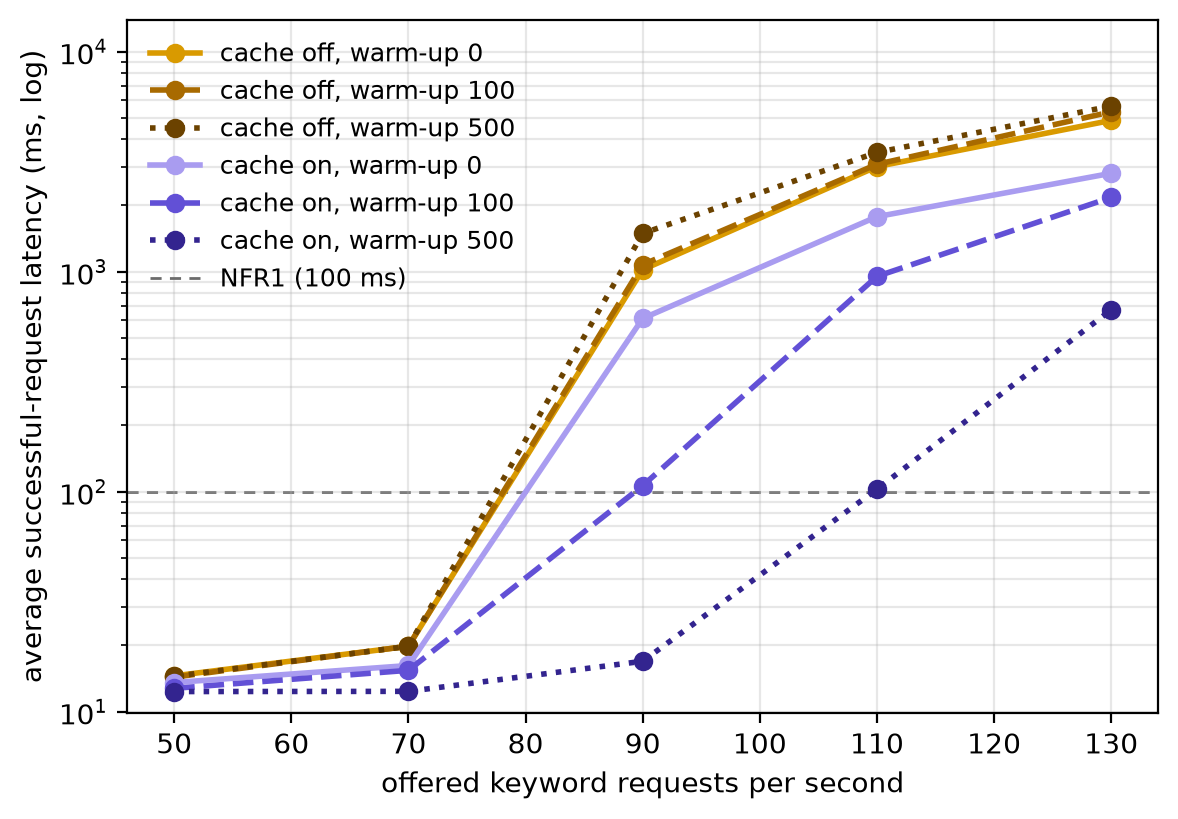
\includegraphics[width=\linewidth]{mac-2026-10-12/phase2/avg-log.png}
    \caption{Phase 2: average latency versus request rate, one server, cache off/on after 0, 100 and 500 warm-up requests.}
    \label{fig:p2avg}
  \end{minipage}\hfill
  \begin{minipage}[t]{0.49\linewidth}
    \centering
    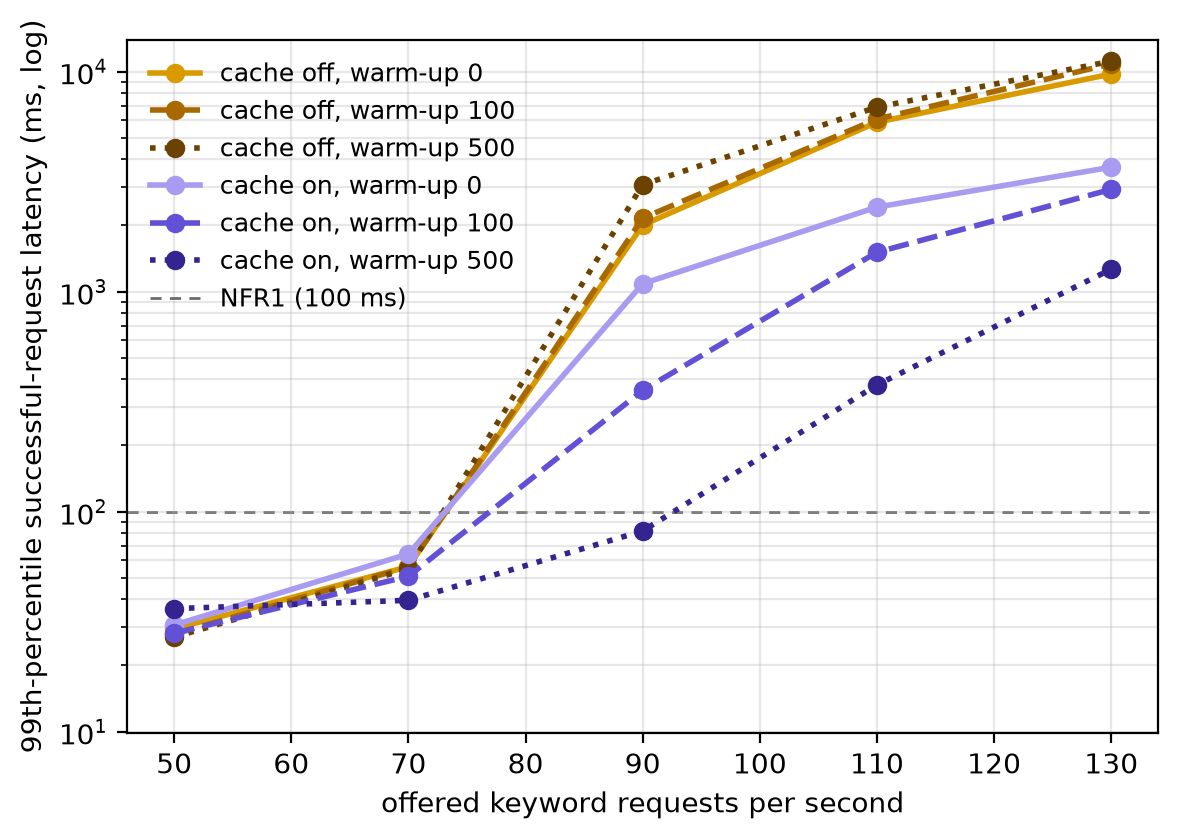
\includegraphics[width=\linewidth]{mac-2026-10-12/phase2/p99-log.png}
    \caption{Phase 2: 99th-percentile latency versus request rate, same conditions as Fig.~\ref{fig:p2avg}.}
    \label{fig:p2p99}
  \end{minipage}
\end{figure}

Up to 70~req/s the latency stays low, about 12--20~ms. With the cache off the server completes at most about 79 requests per second; above this rate the server utilization exceeds 1 and the knee happens, which means more requests arrive than the server can handle: they wait in the server's connection queue, so the latency keeps growing as the run goes. The bottleneck is the single server, which cannot handle all the requests to the system. The cache makes repeated requests faster: by adding the cache with 500 warm-up requests, the maximum request rate that satisfies NFR1 increases from 70~req/s to 90~req/s (99th percentile 56~ms and 82~ms). The 99th percentile rises earlier and higher than the average, because it captures the slowest requests: cache misses on the longest texts and, past the knee, the requests that waited longest in the queue.

% ------------------------------------------------------------------
\section{Phase 3: Scalability and Load Balancing}
% TODO

% ------------------------------------------------------------------
\section{Phase 4: Fault Tolerance}
% TODO

\end{document}
